\documentclass[conf]{new-aiaa}
%\documentclass[journal]{new-aiaa} for journal papers
\usepackage[utf8]{inputenc}

\usepackage{graphicx}
\usepackage{amsmath}
\usepackage{sidecap}
\usepackage[version=4]{mhchem}
\usepackage{siunitx}
\usepackage{longtable,tabularx}
\setlength\LTleft{0pt} 

\title{A Convex Optimal and LQG Control Approach for Quadrotor}

\author{Pádraig Lysandrou
\footnote{Undergraduate Student, Electrical and Computer Engineering, AIAA Student Member \\ A final project for MAE6780: Multivariate Control Theory}}

\affil{Cornell University, Ithaca, New York, 14853}


\begin{document}

\maketitle

\begin{abstract}
In this paper, I present the theory behind and implementation of a neighboring optimal Linear Quadratic Gaussian quadrotor controller with convex optimal guidance trajectories. My LQG solution uses an Extended Kalman Filter for optimal nonlinear estimation. I employ the convex optimization machinery as the guidance algorithm to generate paths of minimum energy consumption. This work is motivated by applications which require efficient use of energy. This includes autonomous delivery, mapping missions, search and rescue, swarm path planning, and many more. The ultimate goal of this project was to design and simulate a functioning LQG controller that follows convex optimal trajectories with high accuracy and amenable to implementation on my own physical autonomous hardware platforms. I would like my solution to be extensible to more complicated tasks in the future.

 The convex optimal guidance works well taking approx (time completion per meter), and the LQG controller converges and accurately tracks trajectories (some metric).
\end{abstract}

\section*{Nomenclature}

{\renewcommand\arraystretch{1.0}
\noindent\begin{longtable*}{@{}l @{\quad=\quad} l@{}}
$A$ & Linearized state space dynamics matrix\\
$B$ & Linearized state space input matrix\\
$C$ & Observation Matrix \\
$\Sigma_{t|t}$ & State covariance matrix at time $t$ with information known at $t$\\
$\mathbf{x}$ & State vector\\
$\mathbf{u}$ & Input vector\\
$\Sigma_w$ &Process noise covariance matrix\\
$\Sigma_v$ & Observation noise covariance matrix \\
$\mathbb{E}[]$ &Expected value operator \\
$\min$ &Minimization operator \\
$Q$ &State penalty matrix \\
$R$ &Input penalty matrix \\
\end{longtable*}}


\clearpage
\begin{doublespace}

\section{Introduction and Theory}
The goal of this project was to design and simulate a functioning LQG controller that follows convex optimal trajectories with high accuracy. Additionally, I wanted the algorithm to be amenable to implementation on my own quadrotor platforms. To reach this goal, I chose a control solution that could be implemented online and would be simple to implement on an embedded system such as an ARM Cortex microcontroller with interrupt service routine timers. Due to Wonham's separation principle, which I will discuss later, the LQG controller can be split up into an optimal regulator (LQR) and an optimal estimator in the form of a Kalman Filter. If both are stable, then the whole control solution is stable. In my implementation, I write my own finite-time-horizon LQR using the Riccati matrix equation. Additionally, I have written my own Extended Kalman Filter (EKF) utilizing nonlinear state propagation via our dynamical equations. For the theory section, I will be covering the quadrotor dynamics, derivation of the LQG controller, introducing convex optimization, and the derivation of my own convex problem proposition.
\subsection{Dynamics of the Quadrotor}
Before we develop the control system, we must first create a dynamic model for the system. The frame of the vehicle is a cross-shape with four motor/propeller combinations, one on each end. In figure \ref{fig:f1}, we see that if we increase the thrust similarly on F1/F2 or F3/F4 the vehicle rolls right or left respectively, as a torque is applied to the system. Additionally we see that if we increase the thrust produced by F4/F1 or F3/F2 the quadrotor pitches forward or backward respectively. The rotor speeds can be increased or decreased to produce a yaw on the vehicle with the conservation of angular momentum. 

\begin{singlespace}
\begin{SCfigure}[1][!h]
	\begin{minipage}{0.5\textwidth}
	\centering
	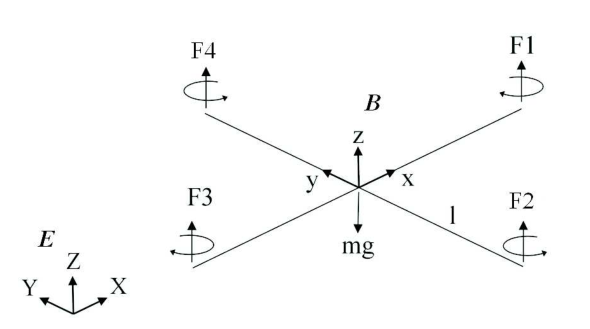
\includegraphics[scale= 0.45]{quad.png}
	\end{minipage}
	\begin{minipage}{0.5\textwidth}
		\begin{tabular}{| l | c |}
		  \hline			
		  $\xi$ & position vector\\
		  $R$ & direction cosine matrix\\
		  $\hat{\omega}$ &skew symmetric angular rate matrix\\
		  $\phi,\theta,\psi$ & roll, pitch, yaw\\
		  $x,y,z$ & inertial position\\
		  $\Omega_i$ & rotor speed\\
		  $I_x,y,z$ & body inertia\\
		  $J_r$ & rotor inertia\\
		  $b$ & thrust factor\\
		  $d$ & drag factor\\
		  $l$ & lever arm\\
		  $g$ & gravitational acceleration\\
		  \hline  
		\end{tabular}
	\end{minipage}
\end{SCfigure}
\begin{figure}[!h]
	\caption{Quadrotor Layout with body fixed frame B and inertial frame E and notation reference}
	\label{fig:f1}	
\end{figure}
\end{singlespace}


\begin{singlespace}
\begin{SCfigure}[1][!ht] 
	\begin{minipage}{0.25\textwidth}
		\begin{equation*}
			\begin{cases}
				& \dot{\xi} = \nu \\
				& m\dot{v} = RF_b \\
				& \dot{R} = R\hat{\omega} \\
				& J\dot{\omega} = -\omega \times J\omega + \tau_a
			\end{cases}
		\end{equation*}
	\end{minipage}
  \begin{minipage}{.4\textwidth}
    \begin{align*}
        &\ddot{x}=(\cos\phi\sin\theta\cos\psi + \sin\phi\sin\psi)\frac{U_1}{m} \\
		&\ddot{y}=(\cos\phi\sin\theta\sin\psi - \sin\phi\cos\psi)\frac{U_1}{m} \\
		&\ddot{z}=(\cos\phi\cos\theta)\frac{U_1}{m} -g \\
		&\ddot{\phi} = \dot{\theta}\dot{\psi}\Big(\frac{I_y - I_z}{I_x}\Big) - \frac{J_r}{I_x}\dot{\theta}\Omega + \frac{l}{I_x}U_2\\
		&\ddot{\theta} = \dot{\phi}\dot{\psi}\Big(\frac{I_z - I_x}{I_y}\Big) - \frac{J_r}{I_y}\dot{\phi}\Omega + \frac{l}{I_y}U_3 \\
		&\ddot{\psi} = \dot{\phi}\dot{\theta}\Big(\frac{I_z - I_y}{I_z}\Big) + \frac{1}{I_z}U_4
    \end{align*}
  \end{minipage}%
  \begin{minipage}{.35\textwidth}
  	\begin{align*}
  		&U_1 = b(\Omega_1^2+\Omega_2^2 + \Omega_3^2 +\Omega_4^2)\\
  		&U_2 = b(\Omega_4^2-\Omega_2^2) \\
  		&U_3 = b(\Omega_3^2-\Omega_1^2) \\ 
  		&U_4 = d(\Omega_2^2+ \Omega_4^2 - \Omega_1^2 - \Omega_3^2) \\ 
  		&\Omega = \Omega_2 + \Omega_4 - \Omega_1 - \Omega_3
  	\end{align*}
  \end{minipage}
\end{SCfigure}
\begin{figure}
	\caption{Governing Nonlinear Coupled Dynamical Equations}
    \label{eq1}
\end{figure}
\end{singlespace}

$U_1, U_2, U_3, U_4,$ and $\Omega$ represent the inputs of the system: total thrust, roll thrust, pitch thrust, and yaw thrust. The first set of equations in the curly braces (\textbf{equations \ref{eq1}}) show the overall simplified dynamics. Once the  thrust is distributed in the inertial frame, we can write the dynamics as the second set of equations shown. These are nonlinear, 6 degree of freedom, coupled dynamical equations. The set of equations on the far right describes these forces in rotor speeds $\Omega_i$. Keep in mind that $U_i$ is not the force from each motor, but follows these equations. Additionally, looking at the simplified second order derivative equations, we see that the translational accelerations are dependent on the attitude dynamics, but the attitude dynamics do not depend on the translational dynamics. Therefore, we can model our dynamics as two subsystems with one dependency. Rewriting in state space form as $\dot{\mathbf{x}}= f(\mathbf{x},\mathbf{U})$, with $\pmb{x}= (x_1 ... x_{12})^T$ as the state vector, we have \textbf{\ref{eq2}}. 
\begin{singlespace}
\begin{SCfigure}[1][!ht] 
	\begin{minipage}{0.3\textwidth}
		\begin{align*}
		\pmb{x}=
			\begin{cases}
				& x_1 = x \\
				& x_2 = \dot{x_1} = \dot{x} \\
				& x_3 = y \\
				& x_4 = \dot{x_3} = \dot{y}\\
				& x_5 = z \\
				& x_6 = \dot{x_5} = \dot{z}\\
				& x_7 = \phi \\
				& x_8 = \dot{x_6} = \dot{\phi}\\
				& x_9 = \theta \\
				& x_{10} = \dot{x}_9 = \dot{\theta}\\
				& x_{11} = \psi \\
				& x_{12} = \dot{x}_{11} = \dot{\psi}
			\end{cases}
		\end{align*}
	\end{minipage}
  \begin{minipage}{.4\textwidth}
  	\[
	\therefore f(\pmb{x},\pmb{U}) =
	\begin{bmatrix}
		& x_2 \\
        &(\cos x_7\sin x_9\cos x_11 + \sin x_7\sin x_11)\frac{U_1}{m} \\
        & x_4 \\
		&(\cos x_7\sin x_9\sin x_11 - \sin x_7\cos x_11)\frac{U_1}{m} \\
		& x_6 \\
		&(\cos x_7\cos x_9)\frac{U_1}{m} -g \\
		& x_8 \\
		&x_{12} x_{10}\Big(\frac{I_y - I_z}{I_x}\Big) - \frac{J_r}{I_x}x_{10}\Omega + \frac{l}{I_x}U_2\\
		& x_{10} \\
		&x_{12} x_8 \Big(\frac{I_z - I_x}{I_y}\Big) - \frac{J_r}{I_y}x_8 \Omega + \frac{l}{I_y}U_3 \\
		& x_{12} \\
		&x_{10} x_8\Big(\frac{I_z - I_y}{I_z}\Big)+ \frac{1}{I_z}U_4
	\end{bmatrix} \]
  \end{minipage}%
\end{SCfigure}
\begin{figure}[!h]
	\caption{State space form of dynamics}
    \label{eq2}
\end{figure}
\end{singlespace}

\subsection{LQG derivation}
We will derive the canonical linear quadratic Gaussian control problem using dynamic programming and backwards induction. First let us describe the system as the following linear time varying state space system. In a later part of this document, we will work with continuous time, linear time-invariant solution. For now we shall propose that $\forall t \in (0 ...T-1)$:
\begin{singlespace}
\begin{align}
& x_{t+1} = A_t x_t + B_t u_t + w_t \\
& y_t = C_t x_t + D_t u_t + v_t
\label{eq3}
\end{align}
\end{singlespace}


Where $\mathbb{E}[w_t]=\mathbb{E}[v_t]=0$. We attribute the cost-to-go structure of $c_t(x_t,u_t) = x_t^T Q_t x_t + u_t^T R_t u_t$ and a terminal cost structure of $c_T(x_T)= x_T^T Q_T x_T$ for $Q_t \geq 0$ positive semidefinite, $R_t > 0$ positive definite to imply convexity in cost. The positive definiteness of $R_t$ gives us required invertibility. Therefore, our cost function is as follows: 
\begin{singlespace}
\begin{equation}
{{\displaystyle J(\mathbf{x},\mathbf{u})=\mathbb {E} \left[{\mathbf {x} }_{N}^{\mathrm {T} }Q_T{\mathbf {x} }_{N}+\sum _{i=0}^{N-1}(\mathbf {x} _{i}^{\mathrm {T} }Q_{i}\mathbf {x} _{i}+\mathbf {u} _{i}^{\mathrm {T} }R_{i}\mathbf {u} _{i})\right]}}
\end{equation}
\end{singlespace}

As an aside, let's notice how we can encode reference tracking objectives, with $\hat{x}$ given as a trajectory, as $c_t(x,u)=||x_t - \hat{x}_t||_2^2$. We see that $||x_t - \hat{x}_t||_2^2 = x_t^Tx_t - 2\hat{x}_t^Tx_t + \hat{x}_t^T\hat{x_t}$ and can generate an augmented state vector as $\tilde{x}=[x_t 1]^T$. This is such that the following exists:
\begin{singlespace}
\begin{equation}
||x_t - \hat{x}_t||_2^2 =
\begin{bmatrix} x_t\\ 1 \end{bmatrix}^T
\begin{bmatrix} I_{nxn} &-\hat{x}_t \\ -\hat{x}_t^T &\hat{x}_t^T\hat{x}_t\end{bmatrix}
\begin{bmatrix} x_t \\ 1\end{bmatrix}
= \tilde{x}_t^T \tilde{Q}_t \tilde{x}_t
\end{equation}
\end{singlespace}

Let's leave this aside for now and see where the backwards inductive dynamic programming approach to solving this function takes us.
\subsubsection{Generating an Optimal Feedback Policy and Deriving the Riccati Equation via Dynamic Programming}
Let's star by evaluating the cost function backwards in time from the finite-time-horizon. The Hamilton-Jacobi-Bellman minimization functions, or optimal costs at each step, will be be referred to with the notation: $V_i^\star$. We will also show this for a linear time-varying system without loss of generality. I will also drop the timing subscripts for the state and input vectors for brevity, but they should be clear from the subscripts found in the function dependencies.
\begin{align}
&\textbf{Stage T:} \quad V_T^\star = \mathbf{x}^TQ_T\mathbf{x}  \\
&\textbf{Stage T-1:} \quad V_{T-1}^\star(\mathbf{x}_{T-1},\mathbf{u}_{T-1}) = \min_{\mathbf{u} \in \mathbb{R}^m} \mathbb {E} \left[\mathbf{x}^TQ_{T-1}\mathbf{x} + \mathbf{u}^TR_{T-1}\mathbf{u} + V_T^\star(A_{T-1}\mathbf{x} + B_{T-1}\mathbf{u} + \mathbf{w}_{T-1}) \right] \\
& = \mathbf{x}^TQ_{T-1}\mathbf{x} + \min_{\mathbf{u} \in \mathbb{R}^m} \mathbb{E} \left[\mathbf{u}^TR_{T-1}\mathbf{u} + (A_{T-1}\mathbf{x} + B_{T-1}\mathbf{u} + \mathbf{w}_{T-1})^TQ_T(A_{T-1}\mathbf{x}+ B_{T-1}\mathbf{u} + \mathbf{w}_{T-1})  \right] \\
& = \mathbf{x}^T(Q_{T-1} + A_{T-1}^TQ_TA_{T-1})\mathbf{x} + \mathbb{E}\left[w_{T-1}^TQ_Tw_{T-1} \right] + \min_{\mathbf{u} \in \mathbb{R}^m} \left[ \mathbf{u}^T(B_{T-1}^TQ_TB_{T-1} + R_{T-1})\mathbf{u} + \mathbf{x}^TA^TQ_TB\mathbf{u} \right]
\label{eqn4}
\end{align}

Here we were able to split apart the equation in deterministic and stochastic quantities. Additionally, we can see that the matrix equation between the $\mathbf{x}^T...\mathbf{x}$ terms is positive semi-definite, and therefore the whole term is convex. The term inside the minimization of equation \ref{eqn4} will be called $f(u)$ going forward. The first term of $f(u)$, between  $\mathbf{u}^T...\mathbf{u}$ is positive definite and the second term is affine in $u$. Therefore, the minimization is quadratic in $u$ and strictly convex due to positive definiteness. Let's minimize by using the gradient:
\begin{singlespace}
\begin{align}
&\nabla_u f(u) = 2(B_{T-1}^TQ_TB_{T-1} + R_{T-1})\mathbf{u} + 2B_{T-1}^TQ_TA_{T-1}\mathbf{x} = \mathbf{0} \\
&\therefore \mathbf{u}^\star = -(B_{T-1}^TQ_TB_{T-1} + R_{T-1})^{-1}(B_{T-1}^TQ_TA_{T-1})\mathbf{x}
\end{align}
\end{singlespace}

Where we have clearly found an optimal, Markovian, feedback policy of the form $\mathbf{u}_{T-1}^\star = L_{T-1}\mathbf{x}_{T-1}$. We can now simplify our cost structure, which will ease our notation for further stages, to the following:
\begin{singlespace}
\begin{align}
& V_{T-1}^\star(\mathbf{x}_{T-1}) = \mathbf{x}^TK_{T-1}\mathbf{x} + \mathbb{E}\left[w_{T-1}^TQ_Tw_{T-1}\right]\\
& \textbf{where} \quad K_{T-1} = A_{T-1}^T (Q_T - Q_TB_{T-1}(B_{T-1}^TQ_TB_{T-1} + R_{T-1})^{-1}B_{T-1}^TQ_T)A_{T-1}
\end{align}
\end{singlespace}

and continuing onward for one more stage
\begin{singlespace}
\begin{align*}
&\textbf{Stage T-2:} \quad V_T^\star(\mathbf{x}_{T-2},\mathbf{u}_{T-2}) =  \min_{\mathbf{u} \in \mathbb{R}^m} \mathbb{E} \left[\mathbf{x}^TQ_{T-2}\mathbf{x} + \mathbf{u}^TR_{T-2}\mathbf{u} + \Xi^TK_{T-1}\Xi \right] + \mathbb{E} \left[ w_{T-1}^TQ_Tw_{T-1} \right]\\
& \text{where the state propagation/prediction is} \quad \Xi = (A_{T-2}\mathbf{x} + B_{T-2}\mathbf{u} + w_{T-2})
\end{align*}
\end{singlespace}

This is unsurprisingly quadratic in $\mathbf{u}$ and again we can obtain from this the optimal policy $\mathbf{u}_{T-2}^\star = L_{T-2}\mathbf{x}_{T-2}$ where $L_{T-2} = -(B_{T-2}^TK_{T-1}B_{T-2} + R_{T-2})^{-1}(B_{T-2}^TK_{T-1}A_{T-2})$. You can continue this backward and inductively prove $L_t, \forall t \in [0 ... T]$. You will get the following
\begin{singlespace}
\begin{align}
& L_{t} = -(B_{t}^TK_{t+1}B_{t} + R_{t})^{-1}(B_{t}^TK_{t+1}A_{t}) \\
& K_T = Q_T\\
& K_t = A_{t}^T (K_{t+1} - K_{t+1}B_{t}(B_{t}^TK_{t+1}B_{t} + R_{t})^{-1}B_{t}^TK_{t+1})A_{t}  \quad \quad \quad \forall t \in [0 ... T-1] \label{eqn5}
\end{align}
\end{singlespace}

You will notice that \ref{eqn5} is the backwards recursive, finite-time-horizon, Riccati Matrix equation. It should be known that now the feedback policy $\mathbf{L}_t$ $\forall t$ can be computed offline and applied to the system. Additionally, for a linear time-invariant system, like ours: $A_t = A$, $B_t = B$, $Q_t = Q$, $R_t = R$ $\forall t$. There are two proofs I will leave out for brevity. The first is that as $T$ approaches infinity, $K$ stays positive semi-definite. The second is the stability margins on the LQG controller. I feel the latter is best summed up by the abstract of John C. Doyle's famous 1978 paper "Guaranteed Margins for LQG regulators" which reads "Abstract -- There are none."

\subsubsection{Derivation of the Optimal Estimator, Kalman Filter}
The second half of the LQG problem is optimal estimation. Our feedback control policy up to now had deterministic state feedback. However, the imperfectly observed system has the feedback policy $u_t^\star = L_t\mathbb{E}[x_t|I_t]$ where $I_t$ is all the sensor information gathered up until that point. Notice that the LQR gain is independent of the noise distribution. Similarly, we will find that the optimal estimate is independent of the control policy. Our objective is to find $x_{t|t}=\mathbb{E}[x_t|I_t]$ given that the state and observation have independent, identically distributed Gaussian additive noise. Throughout the calculation we will keep track of both the state and $\Sigma_{t|t}$ the state covariance matrix. In the first step, we will predict the next state and state covariance matrix ($\mathbf{x}_{t+1|t}$ and $\Sigma_{t+1|t}$) given the current information and the known dynamics of the system. The second step involves filtering this and weighing between the sensor measurements and our own dynamic propagation. Once we generate the estimated state, we can do the algorithm again recursively.

\begin{singlespace}
\begin{align*}
& \textbf{The Prediction Step}\\
&x_{t+1|t} = Ax_{t|t} + Bu_t \\
&\Sigma_{t+1|t} = A\Sigma_{t|t}A^T + G\Sigma_w G^T \\
& \textbf{The Filter Step}\\
&x_{t+1|t+1} = x_{t+1|t} + \Gamma_t (y_{t+1 - C_{t+1}x_{t+1|t}}) \\
&\Sigma_{t+1|t+1} = \Sigma_{t+1|t} - \Gamma_t C_{t+1}\Sigma_{t+1|t} \\ 
& \text{with Kalman Gain:}\quad \Gamma_t= \Sigma_{t+1|t}C_{t+1}^T(C_{t+1}\Sigma_{t+1|t} C_{t+1}^T + H_{t+1}\Sigma_vH_{t+1}^T)   
\end{align*}
\end{singlespace}

However, in the implemented system, I have chosen to use the "Extended" Kalman filter. This is to say that instead of linearly propagating my dynamics, I use the full nonlinear equations ($\therefore x_{t+1|t} = f(\mathbf{x}_{t|t},\mathbf{u})$). However, I still have to linearize the system about a hovering point to be able to use the $A$ matrix in the covariance matrix propagation step.

\subsection{Convex Optimization}
The general form of an optimization problem is to find some $\displaystyle x^\ast \in \mathcal{X}$ such that $\displaystyle f(x^{\ast })=\min\{f(x):x\in {\mathcal {X}}\}$ in a feasible set $\mathcal{X}$. Posing the problem is usually the hard part, and rigorously proving that is convex such that it works with existing computational tools. Many times, the problem is non-convex and tricks like introducing slack variables and other forms of lossless convexification must be employed. Convex optimization problems usually look like:

\begin{singlespace}
\begin{align*}
& \textbf{minimize} &f(x) \\ 
& \textbf{subject to} &g_i(x) \leq 0, \forall i \\
& & h_{i}(x)=0, \forall i
\end{align*}
\end{singlespace}

for convex constraints in $g_i$ and affine equality constraints in $h_i$. I will talk about the problem that I have proposed and the software I used to solve it in the next section.


\section{Procedure}

We will linearize this system of nonlinear equations about a hover point in order to use the LQG solution. Although the Kalman filter will use nonlinear dynamics, we must linearize for our regulator. This means that $\dot{\mathbf{x}} = \nabla_{x,ic}(f(x,u))\mathbf{x} + \nabla_{u,ic}(f(x,u))\mathbf{u}$

5 pages!!
Describe the process  that I took to come to my control solution
describe the simulink blocks and code
with the intention of giving step-by-step instructions to someone

\section{RESULTS}
4 pages
results from the simulations and controllers

Include a description of simulation findings, using diagrams, figures, and numerical data measurements (by means of tables) that provide a convincing argument on the effectiveness and shortcomings of
your chosen multivariable controller, in the context of the original design objectives. 

It may be appropriate to put some of the raw data into Appendices. Plot the results in a meaningful way- “a plot is worth a thousand words,” do NOT underestimate the power of a good plot! Consider using statistical analysis if appropriate when completing a plot. Verify your findings through the theory. Possible causes of error should also be addressed in the concluding paragraph.


\section{Conclusions}
1 paragraph
main contributions, and causes of error, theoretical findings
summary of control performance
what to do in the future

\section{ref}
Be sure to cite any references you used in this lab report using approved IEEE standards. 





\end{doublespace}
\bibliography{sample}
\end{document}
